\documentclass[tikz, margin=5mm]{standalone}

\usepackage[scaled]{helvet}
\renewcommand\familydefault{\sfdefault}
\usepackage[T1]{fontenc}

\definecolor{mycolour}{RGB}{239,131,118}
\usetikzlibrary{fit,positioning,arrows.meta}

\begin{document}
\begin{tikzpicture}[
   font=\sffamily,
   arrow/.style={->,mycolour,line width=1mm},
   box/.style={black,rounded corners=1mm, line width=.75mm},
   circlenode/.style={line width=.75mm}
]

% Input
\node[align=center, text width=4cm] at (-10,-4.25) {\huge Input };
\node[inner sep=0pt] at (-10,-.5) {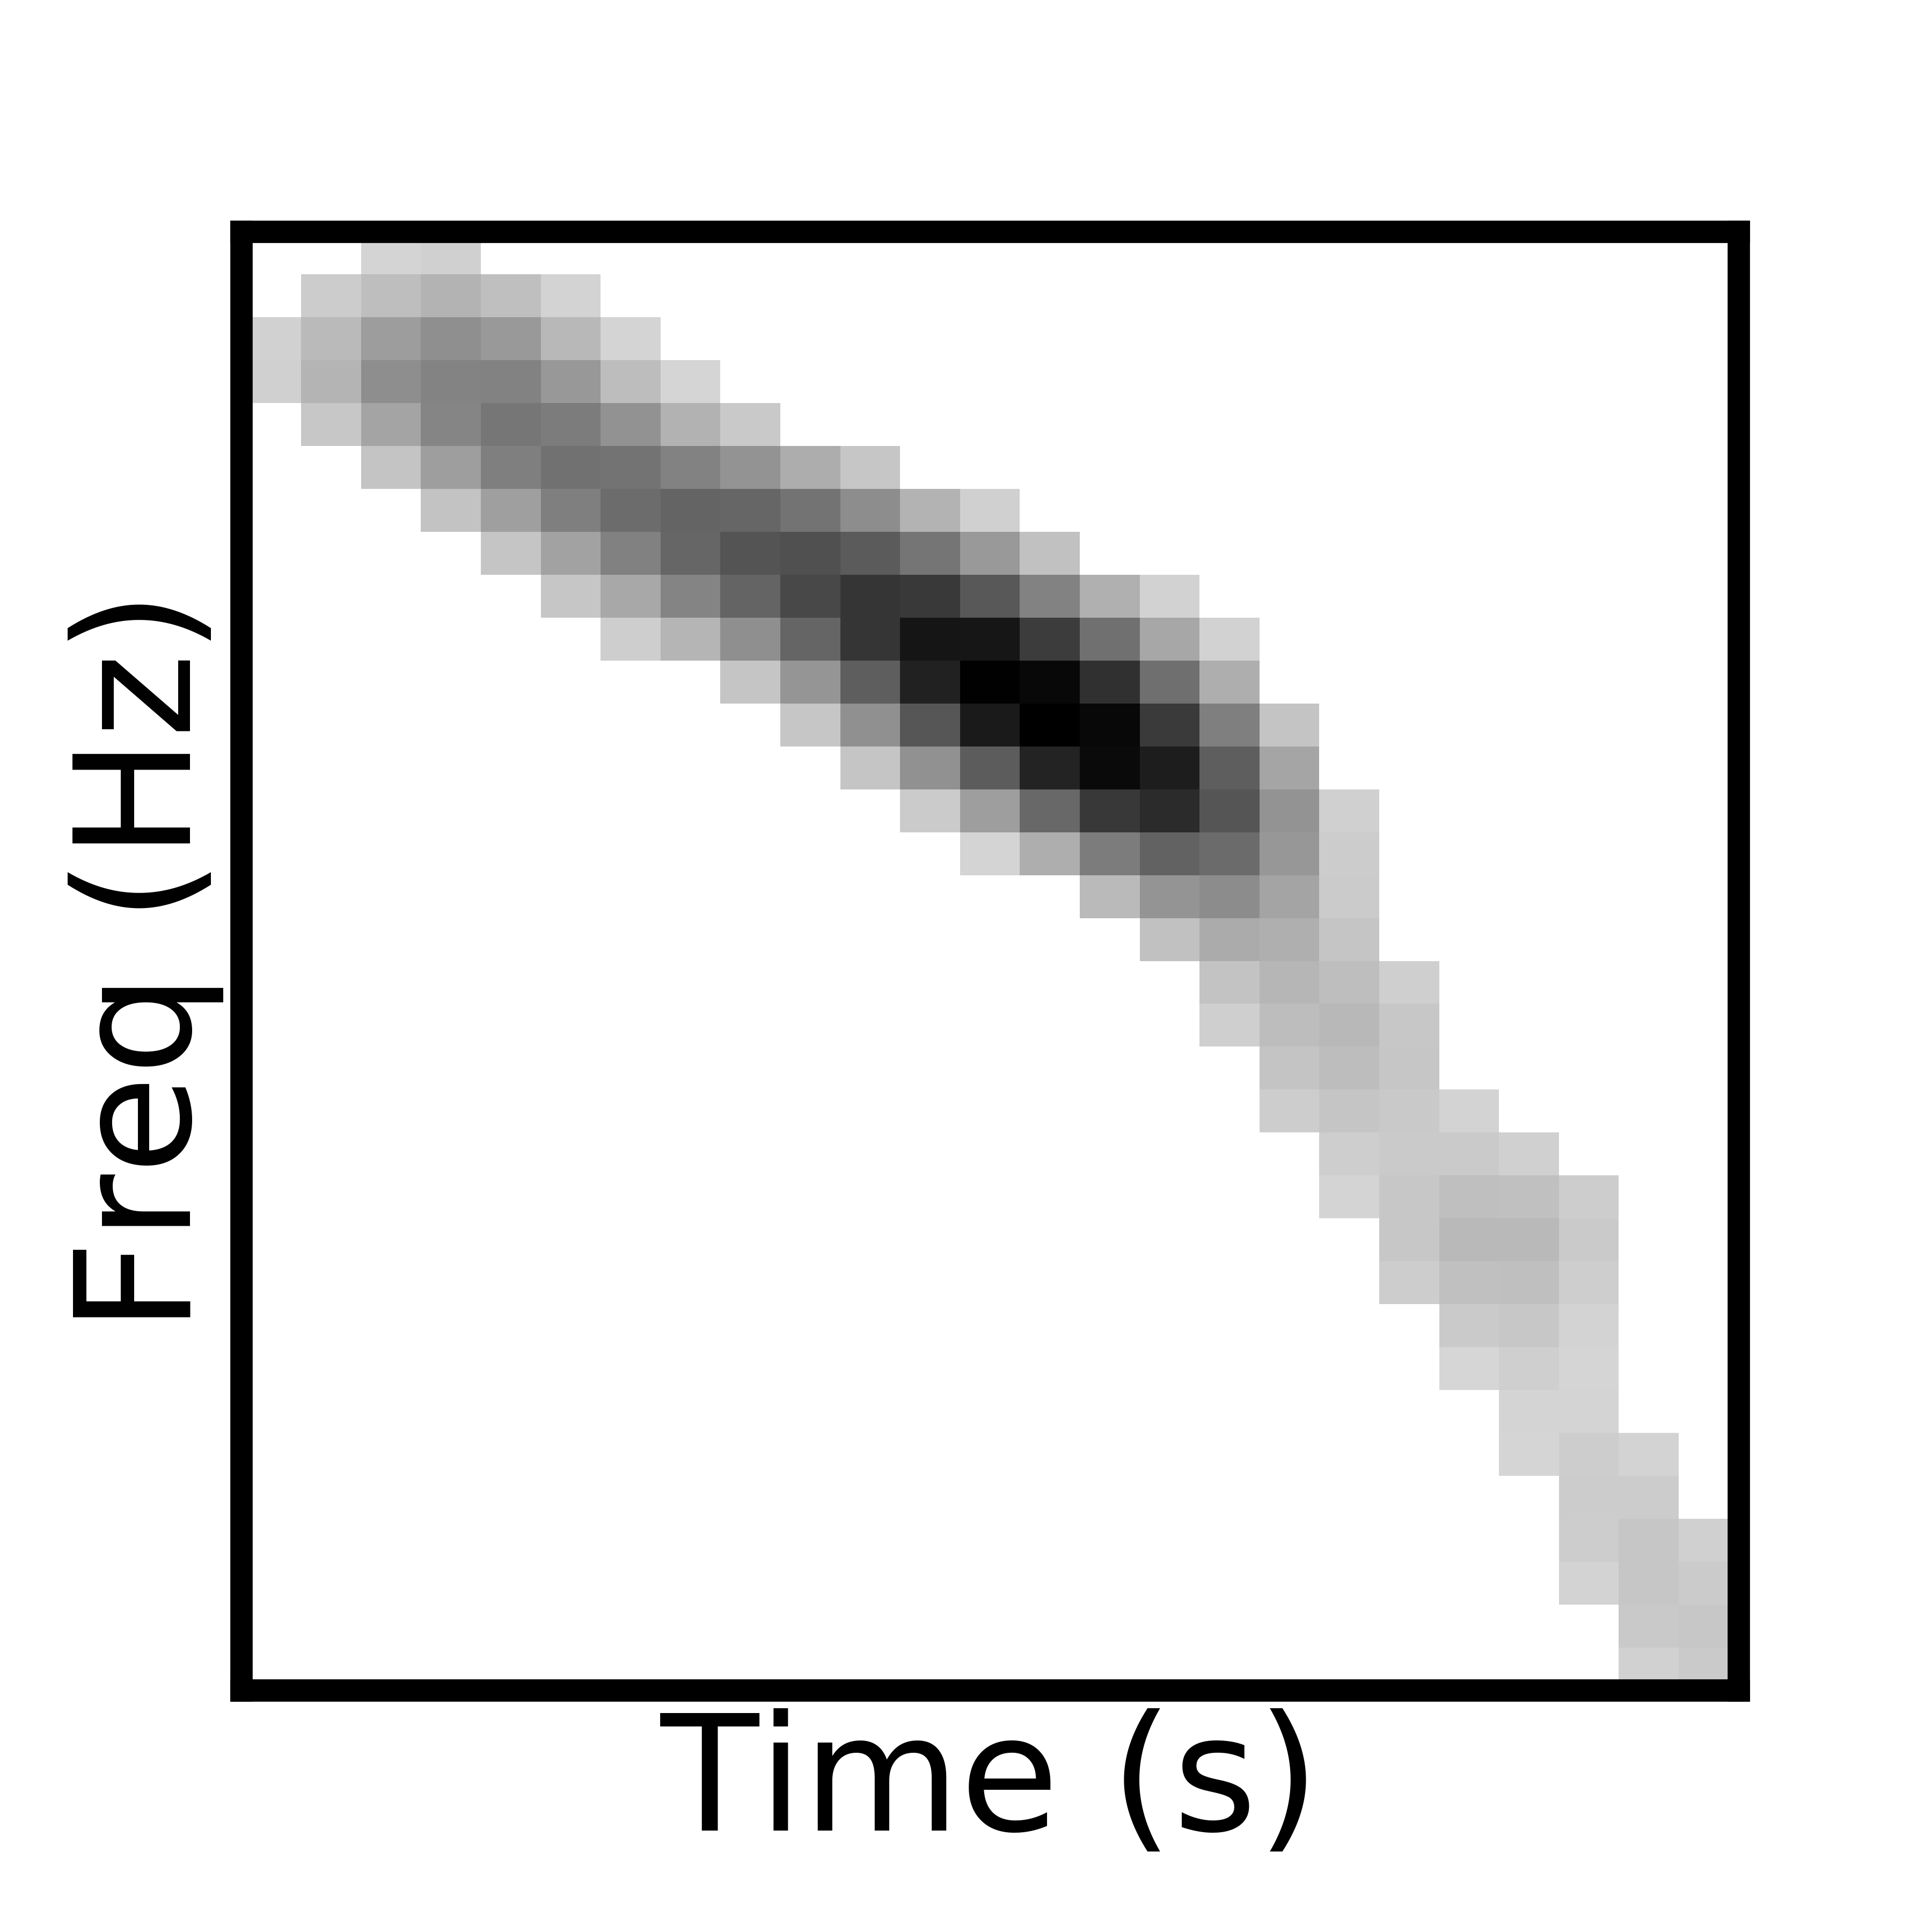
\includegraphics[width=5.75cm, height=5.75cm]{images/spectrogram.png}};
\draw[arrow] (-7,-1,0) -- (-3.5,-1,0) node[midway, above] {\Huge 1.};

% Conv/Pool Layer 1
\node[align=center, text width=4cm] at (-1,-4.25) {\huge Conv/Pool };
\pgfmathsetmacro{\cubex}{3}
\pgfmathsetmacro{\cubey}{3}
\pgfmathsetmacro{\cubez}{4}
\draw[box] (0,0,0) -- ++(-\cubex,0,0) -- ++(0,-\cubey,0) -- ++(\cubex,0,0) -- cycle;
\draw[box] (0,0,0) -- ++(0,0,-\cubez) -- ++(0,-\cubey,0) -- ++(0,0,\cubez) -- cycle;
\draw[box] (0,0,0) -- ++(-\cubex,0,0) -- ++(0,0,-\cubez) -- ++(\cubex,0,0) -- cycle;
\draw[arrow] (2,-1,0) -- (5.5,-1,0) node[midway, above] {\Huge 2.};

% Conv/Pool Layer 2
\node[align=center, text width=4cm] at (8,-4.25) {\huge Conv/Pool };
\pgfmathsetmacro{\cubex}{2}
\pgfmathsetmacro{\cubey}{2}
\pgfmathsetmacro{\cubez}{8}
\draw[box] (8,-1,0) -- ++(-\cubex,0,0) -- ++(0,-\cubey,0) -- ++(\cubex,0,0) -- cycle;
\draw[box] (8,-1,0) -- ++(0,0,-\cubez) -- ++(0,-\cubey,0) -- ++(0,0,\cubez) -- cycle;
\draw[box] (8,-1,0) -- ++(-\cubex,0,0) -- ++(0,0,-\cubez) -- ++(\cubex,0,0) -- cycle;
\draw[arrow] (10.75,-1,0) -- (14.25,-1,0) node[midway, above] {\Huge 3.};

% Conv/Pool Layer 3
\node[align=center, text width=4cm] at (16,-4.25) {\huge Conv/Pool };
\pgfmathsetmacro{\cubex}{1}
\pgfmathsetmacro{\cubey}{1}
\pgfmathsetmacro{\cubez}{8}
\draw[box] (15,-2,0) -- ++(-\cubex,0,0) -- ++(0,-\cubey,0) -- ++(\cubex,0,0) -- cycle;
\draw[box] (15,-2,0) -- ++(0,0,-\cubez) -- ++(0,-\cubey,0) -- ++(0,0,\cubez) -- cycle;
\draw[box] (15,-2,0) -- ++(-\cubex,0,0) -- ++(0,0,-\cubez) -- ++(\cubex,0,0) -- cycle;
\draw[arrow] (17.5,-1,0) -- (21,-1,0) node[midway, above] {\Huge 4.};

% FC Layer 1
\node[align=center, text width=4cm] at (21.75,-4.25) {\huge FC };
\pgfmathsetmacro{\cubex}{.5}
\pgfmathsetmacro{\cubey}{4}
\draw[box] (22,1,0) -- ++(-\cubex,0,0) -- ++(0,-\cubey,0) -- ++(\cubex,0,0) -- cycle;
\draw[arrow] (22.5,-1,0) -- (26,-1,0) node[midway, above] {\Huge 5.};
\draw[circlenode] (21.75,-.5) circle (1.75mm);
\draw[circlenode] (21.75,-1) circle (1.75mm);
\draw[circlenode] (21.75,-1.50) circle (1.75mm);

% FC Layer 2
\node[align=center, text width=4cm] at (26.75,-4.25) {\huge FC };
\pgfmathsetmacro{\cubex}{.5}
\pgfmathsetmacro{\cubey}{3}
\draw[box] (27,.5,0) -- ++(-\cubex,0,0) -- ++(0,-\cubey,0) -- ++(\cubex,0,0) -- cycle;
\draw[arrow] (27.5,-1,0) -- (31,-1,0) node[midway, above] {\Huge 6.};
\draw[circlenode] (26.75,-.5) circle (1.75mm);
\draw[circlenode] (26.75,-1) circle (1.75mm);
\draw[circlenode] (26.75,-1.50) circle (1.75mm);

% Output
\node[align=center, text width=4cm] at (32,-4.25) {\huge Output };
\pgfmathsetmacro{\cubex}{.5}
\pgfmathsetmacro{\cubey}{2.5}
\draw[box] (32,.25,0) -- ++(-\cubex,0,0) -- ++(0,-\cubey,0) -- ++(\cubex,0,0) -- cycle;
\draw[circlenode] (31.75,-.5) circle (1.75mm);
\draw[circlenode] (31.75,-1) circle (1.75mm);
\draw[circlenode] (31.75,-1.50) circle (1.75mm);


\end{tikzpicture}
\end{document}
